% All contribution chapters should follow a similar structure, with a
% mini-introduction and overview at the beginning and a conclusion at the
% end bookmarking a structured presentation of the contribution. This can be
% largely based on your publications.

\chapter{Random Numerical Semigroups}\label{chap:contrib1}

\section{Introduction}

In this Chapter, XXX is presented. Note: to cross-reference to other parts of the document you do so like this - see Section \ref{sec:contrib2:theme1:B}.

Section \ref{sec:contrib1:theme1} discusses Theme 1. Section \ref{sec:contrib1:theme2} discusses Theme 2....

\section{Box Model}\label{sec:contrib1:theme1}

\begin{figure}
\centering
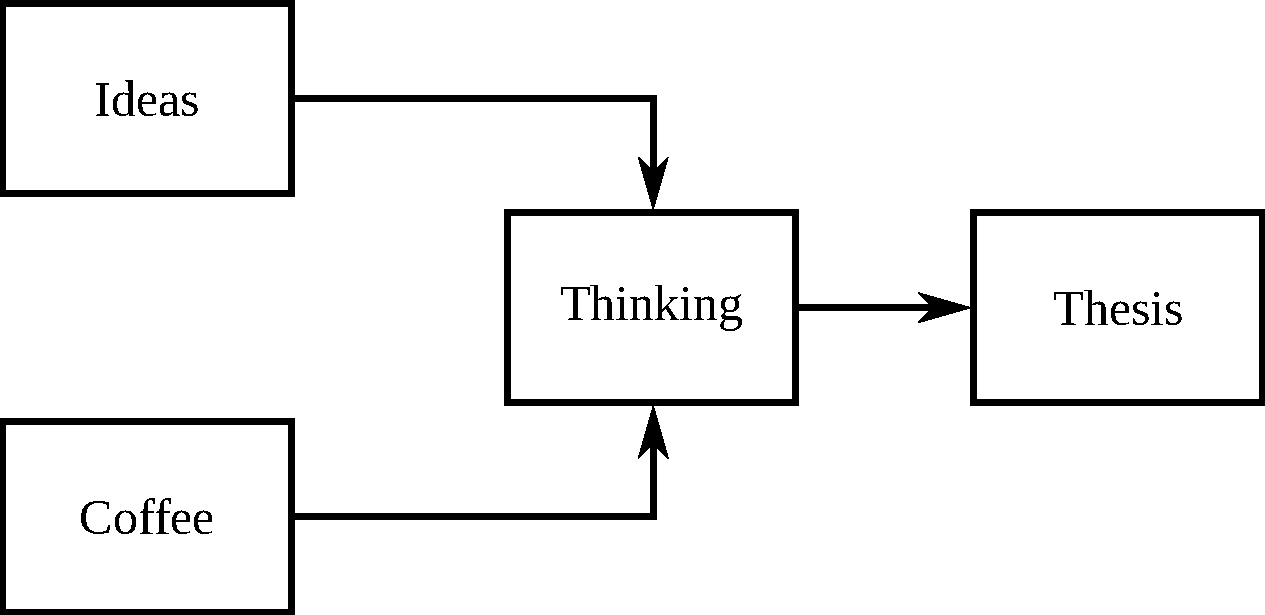
\includegraphics[width=0.8\textwidth]{sample_wide_figure}
\caption{This the approximate process for producing a Thesis. It typically takes 3-4 years.}
\label{fig:phd_life}
\end{figure}

\figurename{} \ref{fig:phd_life} illustrates the key elements of Thesis synthesis. \LaTeX{} will tend to place figures where it wants (they `float' - generally they should be at the top or bottom of a page); you can override the default behaviour if you want, but you probably don't want to bother doing that until after your content is pretty much done. Instead, keep the figures as close as possible to the text; you can tweak this afterwards if you want by adding an option:

\begin{verbatim}
\begin{figure}[htb]
\end{verbatim}

This says put it here, if you can, otherwise at the top, or otherwise at the bottom. BUT I strongly suggest not using {\bf h} as it looks terrible.

Maybe you need an inline URL at this point: Here's one! \url{https://en.wikibooks.org/wiki/LaTeX}.

Mathematics can be inline, for example $x = \int_0^\infty y^2 dy$, or can be in display mode, as shown in \eqref{eqn:example}:

\begin{equation}
\label{eqn:example}
F(x,y,z) = \sqrt{x^{y^z}}
\end{equation}

You probably want to show some of your results in a table, such as \tablename{} \ref{tab:example}.

% Table environment. This is the most difficult thing to get right in LaTeX if you go beyond a simple table like that shown below. Refer to the LaTeX Wikibook for lots of info about creating LaTeX tables (see the toplevel README.md).
\begin{table*}
\centering
\caption{Table captions normally go at the top.}
\label{tab:example}
% Don't leave blank lines in the middle of a floating environment such as table or figure!
% This bit describes how the columns are organised. l, r, c for left, right, centre-justified; p{1cm} or p{0.2\textwidth} for left-justified with fixed width. This is usually best.
\begin{tabular}{p{0.2\textwidth}p{0.3\textwidth}p{0.3\textwidth}}
\toprule
{\bf Left column}	&{\bf $\mu$}	&{\bf $\sigma$}\\
\midrule
Item 1				&0.3			&0.5\\
Item 2				&0.9			&0.4\\
\bottomrule
\end{tabular}
\end{table*}

\begin{figure}
\centering
\subfloat[Confusion]{
	
\includegraphics[height=0.3\textwidth]{confusion}
	\label{fig:confusion}
}
\subfloat[Work]{
	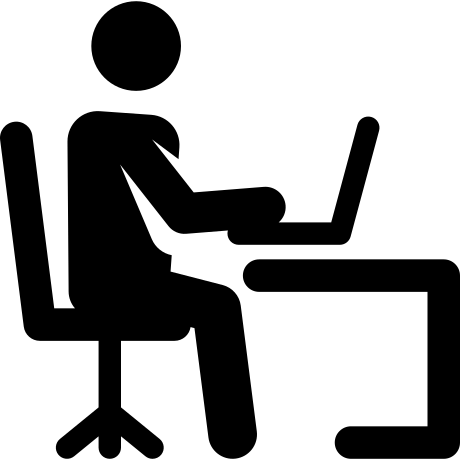
\includegraphics[height=0.3\textwidth]{work}
	\label{fig:work}
}
\subfloat[Exhaustion]{
        
\includegraphics[height=0.3\textwidth]{exhaustion}
        \label{fig:exhaustion}
}
\caption{The stages of the creative process.}
\label{fig:creative_process}
\end{figure}

The basic creative process is shown in \figurename{} \ref{fig:creative_process}. Specifically, \figurename{} \ref{fig:confusion} shows the first step, while \figurename{} \ref{fig:work} and \ref{fig:exhaustion} show the remaining key steps of the procedure.

\subsection{Subtopic A}\label{sec:contrib1:theme1:A}

Algorithm \ref{alg:cap} shows a classical algorithm typeset in \LaTeX{}. This is also a float.

\begin{algorithm}
\caption{An algorithm with caption}\label{alg:cap}
\begin{algorithmic}
\Require $n \geq 0$
\Ensure $y = x^n$
\State $y \gets 1$
\State $X \gets x$
\State $N \gets n$
\While{$N \neq 0$}
\If{$N$ is even}
    \State $X \gets X \times X$
    \State $N \gets \frac{N}{2}$  \Comment{This is a comment}
\ElsIf{$N$ is odd}
    \State $y \gets y \times X$
    \State $N \gets N - 1$
\EndIf
\EndWhile
\end{algorithmic}
\end{algorithm}

\subsection{Results}\label{sec:contrib1:theme1:B}

\subsection{Subtopic C}\label{sec:contrib1:theme1:C}

\section{ER-type model}

We generate a random numerical semigroup with a model similar to the Ërdos-Renyi model for random graphs. 

\begin{definition}
    For $p \in [0, 1]$ and $M \in \NN$, a random numerical semigroup $S(M, p)$ is a probability space over the set of semigroups $S = \langle\mathcal{A}\rangle$ with $\mathcal{A} \subseteq \{1,...,M\}$, determined by
    \[\Pr[n \in \mathcal{A}] = p,\]
    with these events mutually independent.
\end{definition}

\section{Downward model}\label{sec:contrib1:theme2}

Etc. etc.



\section{Conclusion}
